\subsection{Measurements of Particle A}
Particle A was measured on October 11 in 2013. Two of the measurements made retraced their orbits very well, these are referred to as measurement 1 and measurement 2 which can be seen in  in Figure \ref{fig:particleA1} and Figure \ref{fig:particleA1} respectively. Measurement 1 was started with initial condition $n_z \approx 0$ and showed quasi periodic behaviour with a periodic change in amplitude for $n_z$ peaks. Measurement 2 was started with initial condition $n_z \approx 1$ and showed periodic behaviour with very constant $n_z$ peaks. 

Other measurement had reversals where the orbit changed considerably, two examples are seen in Figure \ref{fig:particleA3} and \ref{fig:particleA4}. All measurement data for particle A can be found at \url{goo.gl/jgzSXe} where particle A is referred to as particle 2 from October 11. 


\subsubsection{Measurement 1}
\begin{figure}[H]
\begin{center}
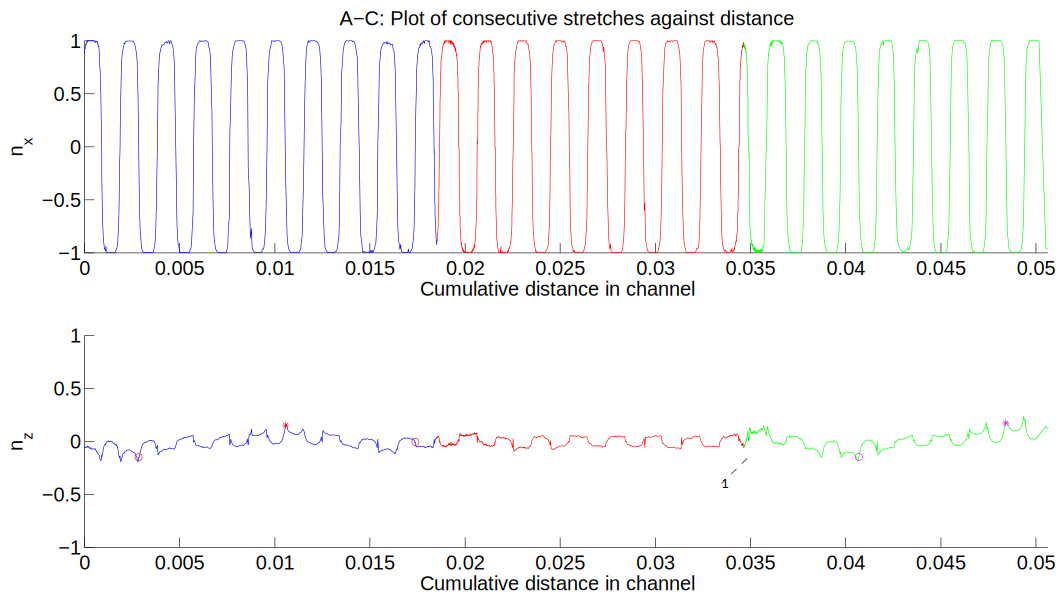
\includegraphics[width=0.7\textwidth]{figures/results/particleA/October_11_Particle_2_run_2_winding.pdf}
\end{center}
\caption{The estimate $n_x$ and $n_z$ components of the particle. Despite being very close to a centre orbit there is limited quasi-periodic behaviour as the peaks stay close to 0. The very flattened peaks compared to a low $n_z$ orbit in \ref{fig:orbitparams} are a result of the width compensation discussed in section \ref{sec:width_compensation}. This particle started $x_0 = 9.8 mm, z_0 = 8.9924 \mu m$ and $D \approx 90\mu$m. This is the same measurement as is used in figure 6.20 in Laas thesis~\cite{alexanderThesis}}
\label{fig:particleA1}
\end{figure}


\subsubsection{Measurement 2}
\begin{figure}[H]
\begin{center}
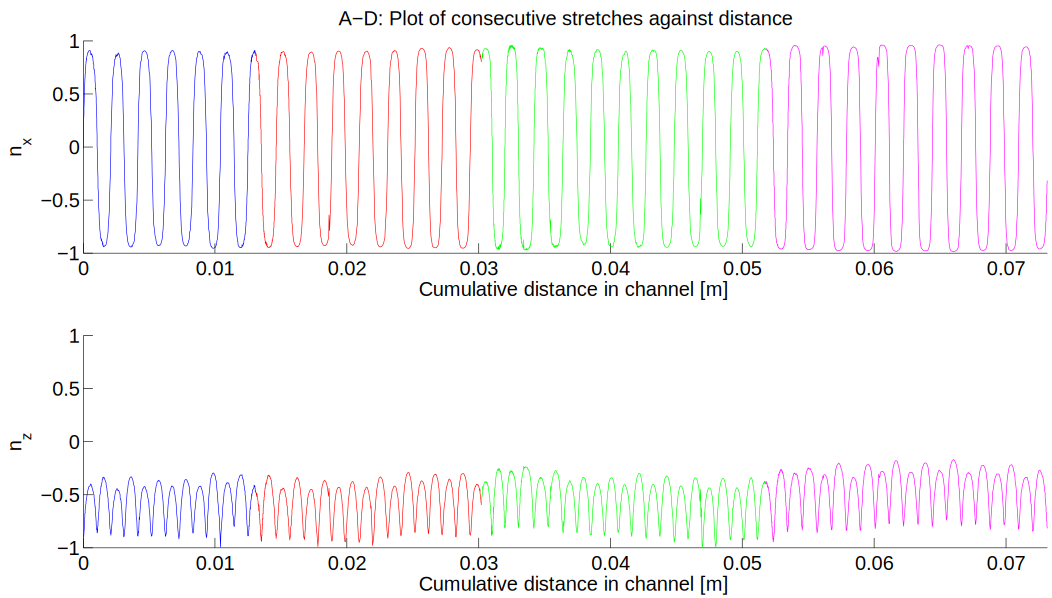
\includegraphics[width=0.7\textwidth]{figures/results/particleA/October_11_Particle_2_run_3_A.pdf}
\end{center}
\caption{The $n_z$ and $n_x$ components for measurement 2 against cumulative distance. The $n_z$ component is consistent ly close to 1 at the peaks and. The particle started at $ x_0 = 26.0 mm, z_0 = 275\mu m, D\approx 105\mu$ m. This figure is the same as can been seen in Laas~\cite{alexanderThesis} figure 6.21}
\label{fig:particleA2}
\end{figure}

\subsubsection{Measurement 3}
\begin{figure}[H]
\begin{center}
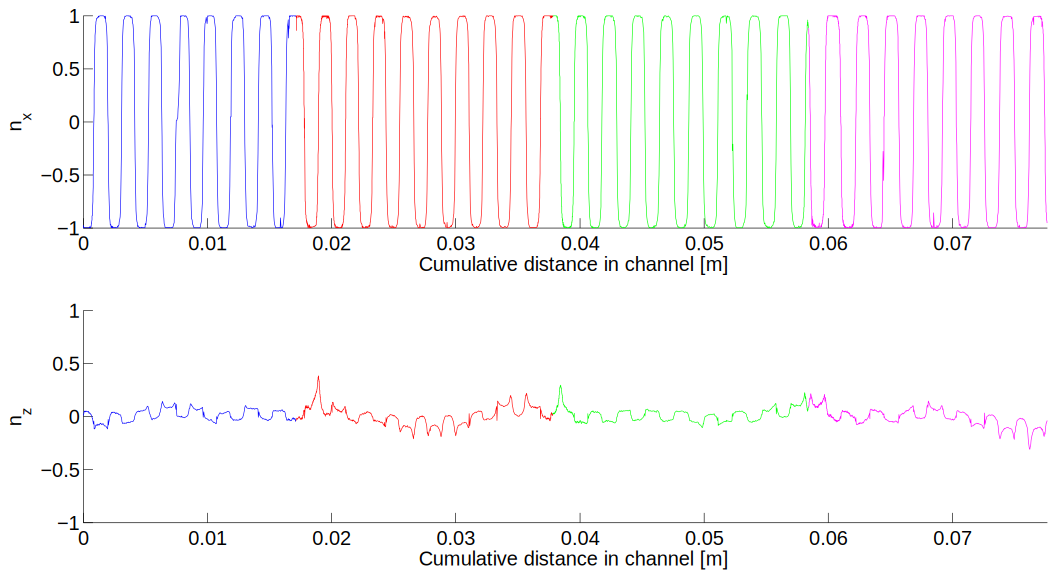
\includegraphics[width=0.7\textwidth]{figures/results/particleA/October_11_Particle_2_run_6_A.pdf}
\end{center}
\caption{The $n_z$ and $n_x$ components for measurement 3 against cumulative distance. The larger peaks that occur after the reversals are not the cause of a tracking error but can be seen clearly in the films. The cause of such a sudden peak and then reverting back to another orbit is not known and we have no good theoretical explanation for it. The reversal of the flow is started when the particle is next to the point marked (3) which is also where there is a change in the orbit. The particle started at $ x_0 = 12.3 mm, z_0 = 160 \mu m, D \approx 100\mu$m. }
\label{fig:particleA3}
\end{figure}



\subsubsection{Measurement 4}
\begin{figure}[H]
\begin{center}
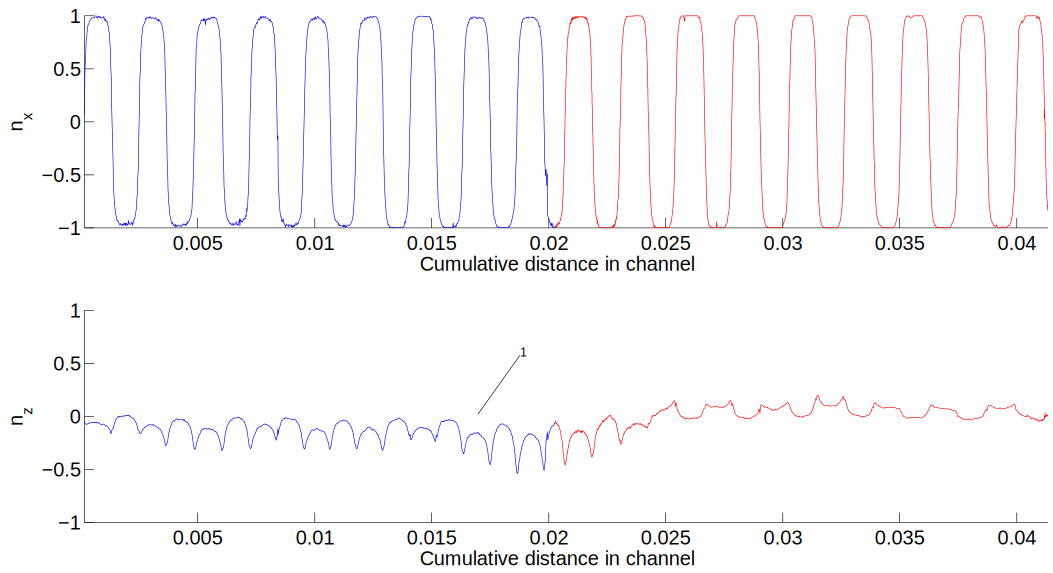
\includegraphics[width=0.8\textwidth]{figures/results/particleA/October_11_Particle_2_run_1_A.pdf}
\end{center}
\caption{The $n_z$ and $n_x$ components for measurement 4 against cumulative distance. The flow is reversed when the particle is at the point marked by (1) and we can see that the peaks around the reversal are larger than for the rest of the measurement. Started at $x_0 = 8.7 mm, z_0 = 16\mu m, D \approx 95\mu$m.}
\label{fig:particleA4}
\end{figure}

\subsubsection{Measurement 5}
\begin{figure}[H]
\centering
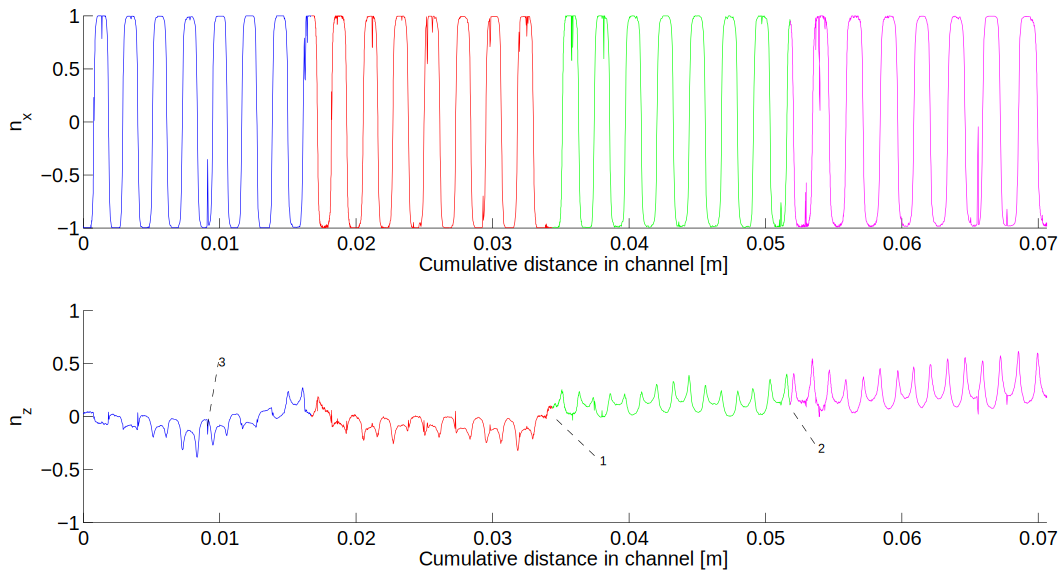
\includegraphics[width=0.8\textwidth]{figures/results/particleA/October_11_Particle_2_run_4_A.pdf}
\caption{The $n_z$ and $n_x$ components for measurement 5 against cumulative distance. At the point marked by (1) $n_z$ changes drastically at the reversal which occurs at the side of the channel closer to the pump. Although there is also some change in the orbit at the reversal marked by (2) it does not move comparably far on the S.O.S. There are a number of small peaks in the data such as the one indicated by (3) which is a consequence is due to insufficient removal of tracking errors, see section \ref{sec:brushing}. The particle started at $x_0 = 10.7 mm, z_0 = 240 \mu m, D \approx 60\mu m$.}
\label{fig:particleA5}
\end{figure}

\subsection{Measurements of Particle B}
Particle B was measured on October 1 2013. Particle B has four measurements for which most reversals showed little change in orbit. These are shown below in Figures \ref{fig:particleB1}, \ref{fig:particleB2}, \ref{fig:particleB3} and \ref{fig:particleB4}. There were also problematic measurements of particle B analogous to those for particle A, but they have not been included in this section for brevity. All measurement data for particle B can be found at \url{goo.gl/jgzSXe} where particle B is referred to as particle 4 from October 1. 

\subsubsection{Measurement 1}
\begin{figure}[H]
\begin{center}
\includegraphics[width=0.7\textwidth]{figures/results/particleB/October_1_Particle_4_run_2_winding.pdf}
\end{center}
\caption{The $n_z$ and $n_x$ components for measurement 1 against cumulative distance. The first two and the last two stretches revert very well. In the reversal between the two good reversals there is a large change in orbit which begins at (1) where the flow is starting to revert. This reversal also occurs at the end of the channel closer to the pump. Starts at $ x_0 = 9.3 mm, z_0 = 35\mu m, D \approx 100\mu m$. This is the same measurement as is used in figure 6.2 and 6.4 in Laas thesis~\cite{alexanderThesis}}
\label{fig:particleB1}
\end{figure}
	


\subsubsection{Measurement 2}

\begin{figure}[H]
\begin{center}
\includegraphics[width=0.7\textwidth]{figures/results/particleB/October_1_Particle_4_run_4_A.pdf}
\end{center}
\caption{The $n_z$ and $n_x$ components for measurement 2 against cumulative distance. The orbit is mostly constant orbit with $n_z \approx 1$ at the peaks. The reversals at (1) and (3) both change the orbit slightly however the difference between the peaks is small and the best matched theoretical orbits in Figure\ref{fig:October1Particle4runs2and2Orbits} are very similar before and after reversals. There is missing data at (2) and (4) where the particle was lost in tracking for some time. The particle started at $x_0 = 28.6 mm, z_0 = 72\mu m, D = \approx 85\mu$ m. This is the same measurement as is used in figure 6.8 in Laas thesis~\cite{alexanderThesis}}
\label{fig:particleB2}
\end{figure}

\subsubsection{Measurement 3}
\begin{figure}[H]
\begin{center}
\includegraphics[width=0.7\textwidth]{figures/results/particleB/October_1_Particle_4_run_5_winding.pdf}
\end{center}
\caption{The $n_z$ and $n_x$ components for measurement 3 against cumulative distance. The initial condition is $n_z \approx 0$ and the sign changes periodically. Started at $x_0 = 2.7 mm, z_0 = 76\mu m, D \approx 90\mu$m. This is the same measurement as is used in figure 6.10 and 6.12 in Laas thesis~\cite{alexanderThesis}}
\label{fig:particleB3}
\end{figure}


\subsubsection{Measurement 4}
\begin{figure}[H]
\begin{center}
\includegraphics[width=0.7\textwidth]{figures/results/particleB/October_1_Particle_4_run_3_winding.pdf}
\end{center}
\caption{The $n_z$ and $n_x$ components for measurement 4 against cumulative distance. While the changes are not large change in $n_z$ there is a periodic variations that could correspond to a sign preserving quasi-periodic orbit. Started at $x_0 = 12.9 mm, z_0 = 21\mu m, D \approx 85\mu$ m}
\label{fig:particleB4}
\end{figure}